\chapter{Approach}
\label{chap:approach}

To evaluate the usefulness of ROS, we set out to build a ROS-based robot control system, targeting the hexapod as its primary hardware platform. A number of increasingly complex requirements were necessary for this system to function correctly.

Throughout, an attitude of code re-use was taken, relying on any existing nodes and packages where possible. It was assumed that these requirements would be otherwise unachievable in this project's time frame without the help of this vast package repository. Packages would be found by simply searching on the web, particularly on the ROS wiki which is used as a centralised resource for all ROS documentation.

%%%%%%%%%%%%%%%%%%%%%%%%%%%%%%%%%%%%%%%%%%%%%%%%%%%%%%%%%%%%%%%%%%%%%%%%%%%%%%%%%%%%%%%%%%%%%%%%%%%%

\section{Requirements}

The requirements for the control system can be divided into four key categories as explained in the following sections.

\subsection{Hardware Operation}

To achieve any real-world interaction, the system had to be capable of interfacing with our target hardware platform. Drivers in some form were required to allow communication to both the servo controller and the RGB-D camera. Ideally, these should transmit and receive on topics using common data types such that they can interact with any generic libraries.

\subsection{Locomotion}

As this robot relies on walking motions for movement, which involves a complex sequence of servo rotations, some abstraction of this process was required. Specifically, it was necessary to be able to control both the linear and angular velocities of the robot without knowledge of these underlying servo movements.

Some calibration process was also necessary. Due to the manner in which the servos connect to their respective joint sections, it is extremely difficult to align them such that they are perfectly straight. A method was required to specify offsets to any positional commands sent to the servo controller on a per-servo basis. Furthermore, to make this process easier some tool to adjust these offsets would be required.

Additionally, a method of manually controlling the robot was needed. This would allow for simple testing before any autonomous behaviour was added as well as acting as a general safety net should anything go catastrophically wrong.

\subsection{Sensing}

By using information received from the attached RGB-D camera, the system had to be be able to interpret the world around it. Specifically, we looked to build up a map of the immediate surrounding area such that it was possible to detect any objects and obstructions.

A method of inferring the position of the robot relative to the rest of the world was also required. Wheeled robots have an advantage in that they are able to apply rotary encoder techniques, allowing them to extrapolate their current position relative to a starting position based on wheel rotations. As this is a walker-style robot, this presented a particularly difficult challenge.

\subsection{Navigation}

Finally, the robot had to be capable of some autonomous behaviour. For this, autonomous navigation was chosen as it would be a stepping stone to any further behaviours. By using the interpreted visual data, the robot had to be able to navigate its environment to reach some particular target while avoiding any obstructions and obstacles where appropriate. To achieve this, we would require a complete working integration of the aforementioned goals.

%%%%%%%%%%%%%%%%%%%%%%%%%%%%%%%%%%%%%%%%%%%%%%%%%%%%%%%%%%%%%%%%%%%%%%%%%%%%%%%%%%%%%%%%%%%%%%%%%%%%

\section{Architecture}

The package concept provided by ROS allows us to divide the control system into a number of dedicated subsystems based on the above requirements. This provides us with a ``separation of concerns'' such that each subsystem only needs to handle one particular task, assuming it has appropriate inputs. For example, the sensing subsystem can assume that it will be provided with valid imagery from the camera thus allowing it to generate a map of the environment. These subsystems can then operate in unison, communicating with each as necessary, to implement the required behaviours. The diagram shown in \autoref{fig:packages} shows an overview of the desired package breakdown. 

\begin{figure}[h!]
    \centering
    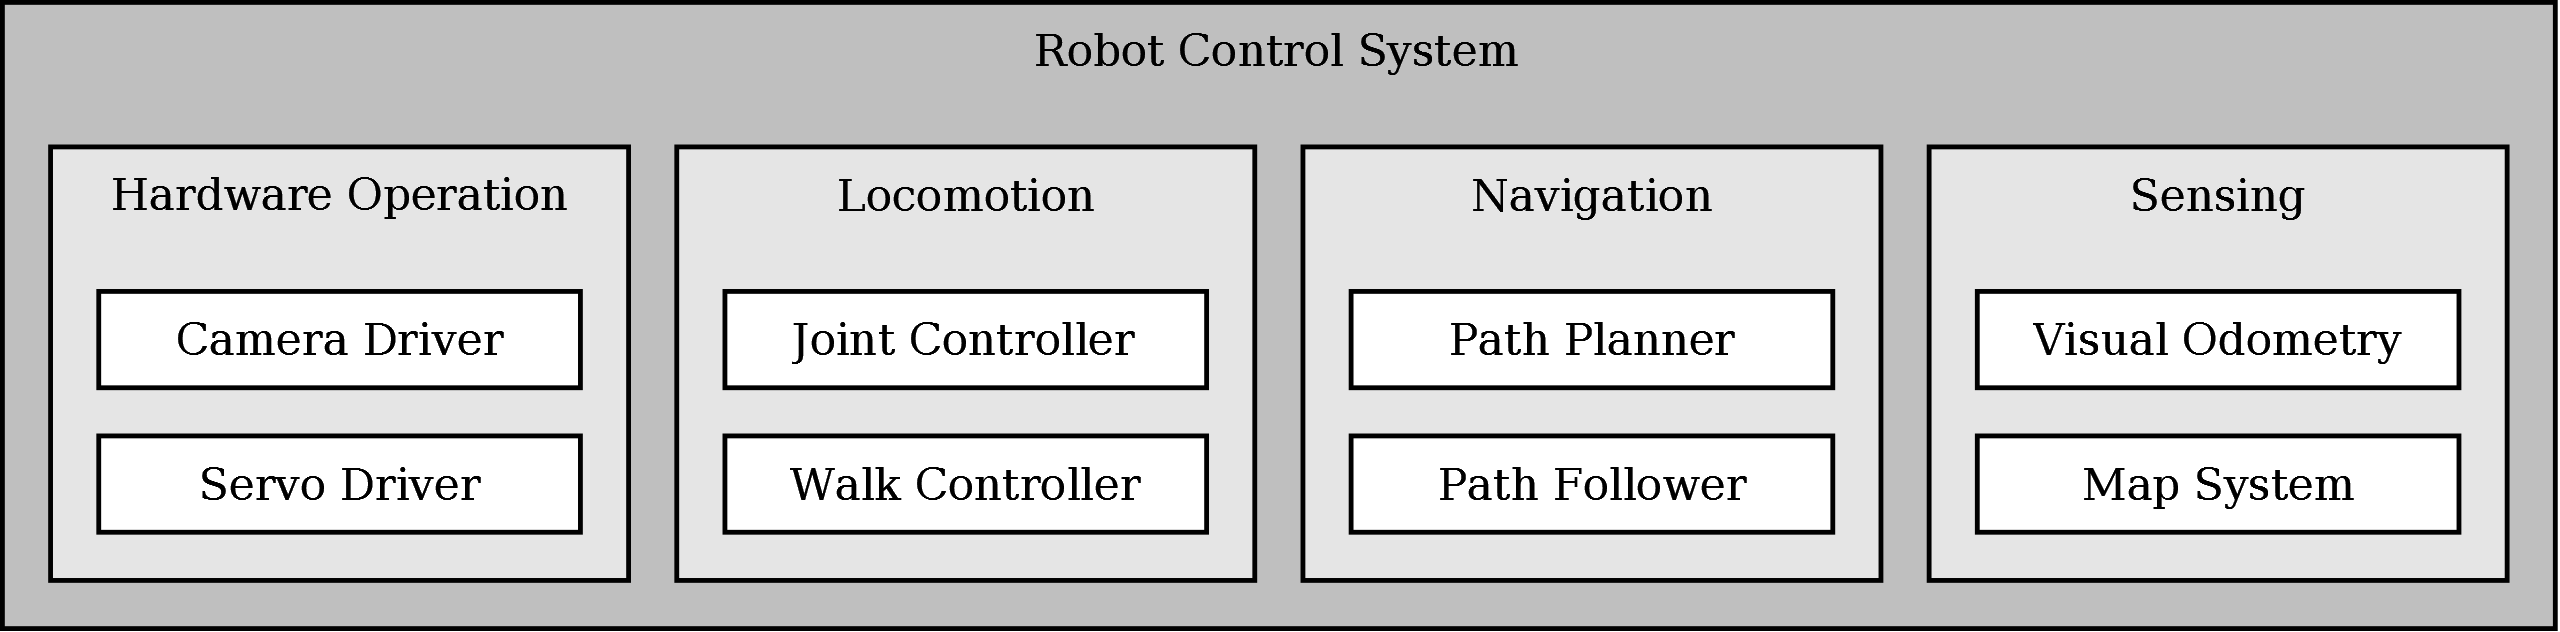
\includegraphics[width=16cm]{packages.png}
    \caption{A diagram showing an overview of the packages layout used in the robot control system.}
    \label{fig:packages}
\end{figure}

The particulars of each subsystem would be implemented as a number of nodes within the package of that subsystem, again only carrying out one singular task of that subsystem providing us with another layer of concern separation. Breaking down tasks in this manner, besides being a standard software development practise, allows us to use as many existing ROS packages as possible. Generic implementations of particular functionalities can be taken and adapted as necessary, as long as we supply them with the correct inputs.